\documentclass[a4paper,12pt]{article}
\usepackage[utf8]{inputenc}
\usepackage{polski}
\usepackage{graphicx}
\usepackage{listings}
\author{Marcin Fabrykowski}
\title{Modelowanie procesów fizycznych\\Lab 06}
\begin{document}
\maketitle
\newpage
\section{Opis problemu}
Celem ćwiczenia jest zamodelowanie bilansu radiacyjnego Ziemi w oparciu o prosty model zaprezentowany na wykładzie
\section{Metoda 1}
Przy użyciu metody pierwszej, nie uwzględniającej wpływu atmosfery, otrzymałem wynik 366K
\section{Metoda 2}
W metodzie tej uwzględniamy wpływ atmosfery. Obliczenia przeprowadzamy dla zakresu stałem słonecznej w zakresie 0.8S do 1.2S.\\
Wykresy temperatury atmosfery i powierzchni przedstawiono na rys \ref{fig:zad2}.
\begin{figure}
\hspace{-7em}
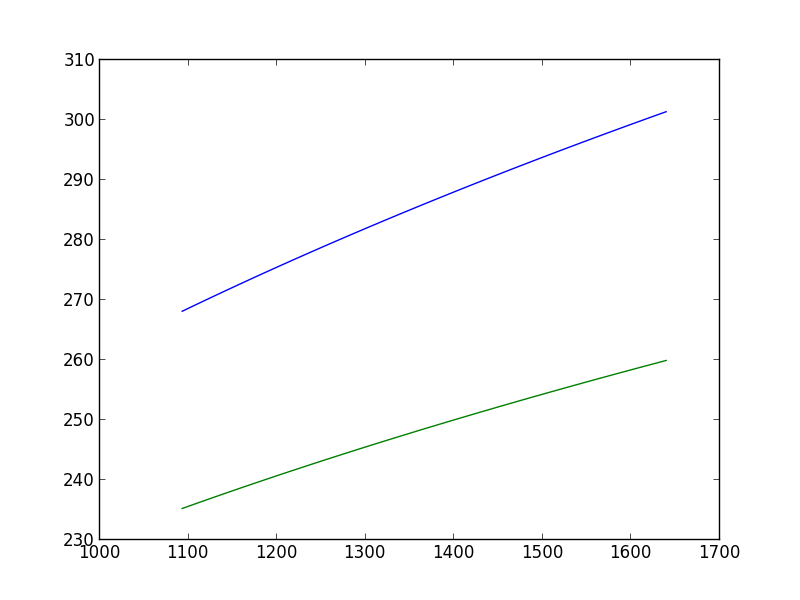
\includegraphics{zad2}
\caption{Zależność temperatur od stałej słonecznej}
\label{fig:zad2}
\end{figure}
\section{Kod programu}
\footnotesize
\lstinputlisting[language=python,tabsize=2]{lab06.py}
\normalsize
\end{document}
